% PyBaMM Battery Modelling Conference 2026 --- 1-page abstract.
% Author: Krishna Chaitanya Vaddepally, Turno (Blubble Pvt. Ltd.)
% Deadline: 2026-07-15 UTC.
%
% Formatted per the PyBaMM 2025 book-of-abstracts template:
% Arial/Helvetica 12 pt minimum, centred bold title, presenting author
% underlined, centred italic affiliation, flowing narrative paragraphs
% without section headings, Figure 1 caption, numbered References.
% Compile with: cd paper && latexmk -pdf pybamm_conf_abstract_v6_final.tex
\documentclass[12pt,a4paper]{article}

\usepackage[T1]{fontenc}
\usepackage{amsmath,amssymb}
\usepackage{helvet}   % Arial-equivalent sans-serif; PyBaMM template accepts Arial >= 12 pt
\renewcommand{\familydefault}{\sfdefault}

\usepackage[a4paper,top=1.5cm,bottom=1.5cm,left=1.8cm,right=1.8cm]{geometry}
\usepackage{graphicx}
\usepackage{caption}
\captionsetup{font=footnotesize,labelfont=bf,labelsep=colon,skip=4pt}
\usepackage{microtype}
\usepackage[hidelinks]{hyperref}
\usepackage{enumitem}

\pagestyle{empty}
\setlength{\parindent}{0pt}
\setlength{\parskip}{0.30em}

\begin{document}
\enlargethispage{5\baselineskip}

\begin{center}
{\bfseries\large Cross-supplier LFP state-of-health forecasting using a\\
PyBaMM-trained neural operator}\\[0.4em]
\underline{Krishna Chaitanya Vaddepally}\\
\emph{Turno (Blubble Pvt.\ Ltd.), Bengaluru, India}\\
krishna.vaddepally@turno.club\\[0.2em]
{\footnotesize Theme: Data-driven Methods \textbullet\ Presentation preference: Oral (poster acceptable)}
\end{center}
\vspace{0.2em}

The reuse of retired lithium iron phosphate (LFP) cells is limited by the
time and cost required to determine their future degradation behaviour.
Conventional lifetime assessment requires extended cycling, while purely
empirical models often transfer poorly between cells with different
designs and manufacturing histories. We present a physics-conditioned
neural operator that forecasts the state-of-health (SoH) trajectory of
second-life LFP cells from a compact diagnostic characterisation.

The workflow first estimates cell-specific electrochemical parameters
from short rest-voltage, pulse-response and partial capacity
measurements (approximate open-circuit voltage inversion, pulse-derived
series resistance, and an initial-capacity anchor). These parameters
condition a Neural ODE~[2] that predicts SoH as a function of cycle
number. The operator is trained using 490 degradation trajectories
generated in PyBaMM~[1] by perturbing five parameters governing
solid-electrolyte-interphase (SEI) growth (rate, molar volume, solvent
diffusivity), lithium plating, and negative-electrode loss of active
material, around seven experimentally characterised anchor cells drawn
from three commercial LFP suppliers (CALB, EVE, REPT). A
censored-likelihood objective allows trajectories that do not reach the
selected end-of-life threshold within the simulation horizon to
contribute to training.

Evaluation was performed on three held-out experimental cells, one per
supplier, using only the nearest-supplier-anchor parameter vector as a
prior (no per-cell degradation-curve fit). The model achieved in-window
SoH root-mean-square errors of 0.53, 1.10 and 0.97 percentage points on
the actual (nameplate-normalised) SoH scale for the CALB, EVE and REPT
cells respectively (Figure~\ref{fig:heldout}). The standard deviation of
the cell-level errors was 0.24 percentage points, providing preliminary
evidence of consistent performance across the three evaluated commercial
LFP cell families. We hypothesise that conditioning on physically
interpretable parameters, rather than raw characterisation traces,
contributes to the observed transferability.

\begin{figure}[h]
  \centering
  \IfFileExists{figures/heldout_soh_overlay.pdf}{%
    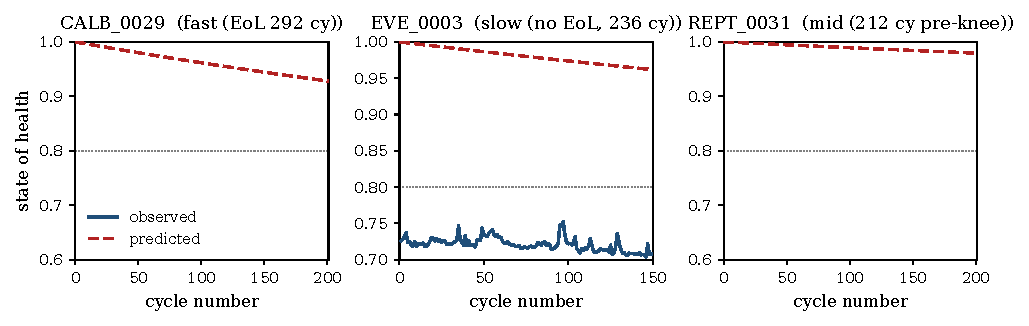
\includegraphics[width=0.88\textwidth]{figures/heldout_soh_overlay.pdf}%
  }{%
    \fbox{\parbox[c][1.2cm][c]{0.95\textwidth}{\centering\footnotesize
      [placeholder: figures/heldout\_soh\_overlay.pdf]}}%
  }
  \caption{Observed vs forecast SoH on three held-out cells (one per
  supplier). SoH is expressed as discharge capacity divided by nameplate
  capacity, so second-life cells enter the plot below 1.0. The operator
  forecast (red dashed) is anchored at the observed first-cycle SoH; no
  cell-specific degradation fit is used. In-window SoH RMSE: 0.53, 1.10,
  0.97 percentage points; cell-level std = 0.24\,pp.}
  \label{fig:heldout}
\end{figure}

The proposed framework connects short experimental diagnostics,
PyBaMM-generated lifetime simulations and computationally efficient
trajectory forecasting. Ongoing work will expand the number of
experimental anchor and validation cells, quantify forecast uncertainty,
and evaluate end-of-life-cycle prediction under application-specific
second-life thresholds.

\vspace{0.2em}
\textbf{References:}
\begin{enumerate}[leftmargin=1.3em,itemsep=0.12em,topsep=0.1em]
  \item V.\ Sulzer, S.\,G.\ Marquis, R.\ Timms, M.\ Robinson, S.\,J.\ Chapman,
  ``Python Battery Mathematical Modelling (PyBaMM)'',
  \emph{Journal of Open Research Software} \textbf{9} (2021), 14.
  \item R.\,T.\,Q.\ Chen, Y.\ Rubanova, J.\ Bettencourt, D.\ Duvenaud,
  ``Neural Ordinary Differential Equations'',
  \emph{Advances in Neural Information Processing Systems} (2018).
\end{enumerate}

\end{document}
